\documentclass[twoside]{report}

\newcommand{\RootPath}{./}
\newcommand{\MyPath}{\RootPath Boostan/tex/}

\usepackage{adjustbox}
\usepackage{ptext}
\usepackage{algorithm}
\usepackage{algorithmic}
\usepackage{listings}
\usepackage{media9}
\usepackage{tabularx}
\usepackage{float}

% قالب بستان؛ بارگذاری بسته‌ها و تنظیمات آن (شامل xcolor با گزینه‌هایش)
\input{\MyPath Boostan-Thesis}

\usepackage{tikz}
\usetikzlibrary{arrows.meta,positioning}

% رنگ و تنظیمات کد پس از بارگذاری قالب
\definecolor{codeColor}{rgb}{0.95,0.95,0.95}
% فونت فارسی بدنه گلوله‌ی فهرست‌ها را ندارد — گلوله از فونت لاتین
\renewcommand{\labelitemi}{\lr{\textbullet}}
% خط تیره‌ی بلند (—) در فونت فارسی گلیف ندارد — از فونت لاتین
\newcommand{\pdash}{\lr{\textemdash}}
\lstset{
	backgroundcolor=\color{codeColor},
	basicstyle=\ttfamily\footnotesize,
	keywordstyle=\color{blue},
	commentstyle=\color{gray},
	stringstyle=\color{brown},
	showstringspaces=false,
	numbers=left,
	numberstyle=\tiny\color{gray},
	breaklines=true,
	frame=single,
	rulecolor=\color{black},
}

%واژه‌های خود را در فایل words وارد کنید، و در ضمن اختصارات را نیز در abbre وارد کنید.
% واژه‌نامه (glossary) — با \gls{کلید} در متن استفاده می‌شود.
\newword{UiAutomation}{UI Automation}
{خودکارسازی رابط کاربری}{}

\newword{PageObject}{Page Object}
{شیء صفحه}{شیءهای صفحه}

\newword{StableIdentifier}{Stable Identifier}
{شناسه پایدار}{شناسه‌های پایدار}

\newword{ReadoutContract}{Readout Contract}
{قرارداد خوانش}{قراردادهای خوانش}

\newword{Fixture}{Fixture}
{داده‌ی پایه‌ی تست}{داده‌های پایه‌ی تست}

\newword{DriverFactory}{Driver Factory}
{کارخانه‌ی درایور}{}

\newword{HandleCache}{Handle Cache}
{نهانگاه دسته‌ها}{}

\newword{SmokeTest}{Smoke Test}
{تست دود}{تست‌های دود}

\newword{RegressionTest}{Regression Test}
{تست بازگشت}{تست‌های بازگشت}

\newword{HeadlessRun}{Headless Run}
{اجرای بی‌سر}{اجرای‌های بی‌سر}

\newword{UiVirtualization}{UI Virtualization}
{مجازی‌سازی رابط کاربری}{}

\newword{QualityMetric}{Quality Metric}
{سنجه‌ی کیفیت}{سنجه‌های کیفیت}

\newword{PhaseAttach}{Phase Attach}
{اتصال فازی}{}

\newword{TestSuites}{Test Suite}
{سوییت}{سوییت‌های}
\newacronym{E2E}{E2E}{End-to-End}

\newacronym{DSL}{DSL}{Domain-Specific Language}

\newacronym{POM}{POM}{Page Object Model}

\newacronym{UIA}{UIA}{UI Automation}

\newacronym{WAD}{WAD}{WinAppDriver}

\newacronym{API}{API}{Application Programming Interface}

\newacronym{GUI}{GUI}{Graphical User Interface}

\newacronym{CI}{CI}{Continuous Integration}

\newacronym{CD}{CD}{Continuous Delivery}

\newacronym{SUT}{SUT}{System Under Test}

\newacronym{KPI}{KPI}{Key Performance Indicator}

\newacronym{CSV}{CSV}{Comma-Separated Values}

\newacronym{QML}{QML}{Qt Modeling Language}

\title{طراحی و پیاده‌سازی چارچوب تست \lr{E2E} برای نرم‌افزارهای مبتنی بر \lr{Qt C++}}
\faculity{دانشکده مهندسی کامپیوتر}
\group{نام گروه}
\author{علیرضا بیات خانی}
\authorCode{99521136}
\forwhat{پایان‌نامه کارشناسی}
\field{در رشته‌ مهندسی کامپیوتر}
\logofile{Logo/Fa}
\logoScale{0.25\linewidth}
\supervisor{دکتر ابوالفضل دیانت}
\date{پاییز 1405}

\graphicspath{{./Pic/}}

\begin{document}
\pagenumbering{gobble}
\thesisStyleO
\newpage
\Godpage
\newpage
\clearpage\newpage
\begin{center}
\vskip 1.5cm
\Large
\typefontR{\Large
	تأییدیه هیئت داوران جلسه دفاع از پایان‌نامه / رساله
}
\end{center}
\vspace{1.5cm}
\makeatletter
\noindent\textbf{نام دانشکده:} \@faculity

\noindent\textbf{نام دانشجو:} \@author

\noindent\textbf{عنوان پایان‌نامه:} \@title

\noindent\textbf{تاریخ دفاع:} \@date

\noindent\textbf{رشته:} \@field

\noindent\textbf{گرایش:} \@group

\vspace{1cm}
\begin{center}
\setlength{\tabcolsep}{15pt}
\begin{tabular}{|c|c|c|c|c|}\hline
\textbf{ردیف} & \textbf{سمت} & \textbf{نام و نام‌خانوادگی} & \textbf{دانشگاه یا مؤسسه} & \textbf{امضا} \\\hline  
1 & استاد راهنما &  
\@supervisor &
دانشگاه علم و صنعت ایران &  
\\\hline 
2 & استاد مدعو خارجی & دکتر ........  & دانشگاه .........  &  
\\\hline  
3 & استاد مدعو داخلی & دکتر ........... & دانشگاه علم و صنعت ایران  &  
\\\hline
\end{tabular}
\end{center}
\makeatother



















\clearpage\newpage
\makeatletter

\begin{center}
{\LARGE{\textbf{تأییدیه صحت و اصالت نتایج}}}\\*[1cm]
باسمه تعالی
\end{center}


این‌جانب
\textbf{\@author}
به شماره دانشجویی
\textbf{\@authorCode}
دانشجو رشته \textbf{مهندسی کامپیوتر} مقطع تحصیلی \textbf{کارشناسی }تایید می‌نمایم که کلیه مندرجات در این پایان‌نامه حاصل کار پژوهشی اینجانب تحت نظارت و راهنمایی عضو هیأت علمی دانشگاه علم و صنعت ایران، بدون هرگونه دخل و تصرف انجام گرفته و موارد نسخه‌برداری شده از آثار دیگران، مطابق مقررات و ضوابط ارجاع داده شده و ویژگی‌های کامل منابع را در فهرست منابع ذکر کرده‌ام. این پایان‌نامه پیش‌تر برای احراز هیچ مدرکی ارائه نگردیده است. 

در صورت اثبات خلاف مندرجات فوق، به تشخیص دانشگاه مطابق با ضوابط و مقررات حاکم (قانون حمایت از حقوق مولفان و منصفان و قانون ترجمه، تکثیر و نشریات و آثار صوتی، ضوابط و مقررات آموزشی و پژوهشی، انضباطی و غیره) با اینجانب رفتار خواهد شد و حق هرگونه اعتراض در خصوص احقاق حقوق مکتسب و تشخیص و تعیین تخلف و مجازات را از خویش سلب می‌نمایم. در ضمن، مسئولیت هرگونه پاسخگویی به اشخاص اعم از حقیقی و حقوقی و مراجع ذی‌صلاح (اعم از اداری و قضایی) به عهده اینجانب خواهد بود و دانشگاه هیچ گونه مسئولیتی در این خصوص نخواهد داشت. 

کلیه نتایج و حقوق حاصل از این پایان‌نامه متعلق به دانشگاه علم و صنعت ایران است. هرگونه استفاده از نتایج علمی و عملی و واگذاری اطلاعات به دیگران یا چاپ و تکثیر، نسخه‌برداری، ترجمه و اقتباس از این پایان‌نامه بدون موافقت کتبی دانشگاه علم و صنعت ایران ممنوع است. نقل مطالب با ذکر منبع بلامانع است. 


\vskip 1cm
\begin{flushleft}
\begin{table}[H]
\raggedright
\begin{tabular}{rr}
نام و نام‌خانوادگی دانشجو: &
\@author \\*[5mm]
تاریخ: &
\@date \\*[5mm]
امضای دانشجو: &
\\
\end{tabular}
\end{table}
\end{flushleft}
\makeatother

\chapter*{چکیده}

تست خودکار رابط کاربری برای نرم‌افزارهای مبتنی بر
\lr{Qt C++}
تا امروز عمدتاً به ابزارهای تجاری محدود بوده و ابزارهای متن‌باز موجود، تنها زیرساخت خام (درایور و پروتکل) را فراهم می‌کنند. این پایان‌نامه طراحی و پیاده‌سازی یک چارچوب تست سرتاسری
\lr{\gls{E2E}}
متن‌باز برای برنامه‌های دسکتاپ مبتنی بر
\lr{Qt}
در بستر ویندوز را گزارش می‌کند. چارچوب بر زیرساخت
\lr{WinAppDriver}/\lr{Appium}
استوار است و با پنج لایه‌ی معماری \pdash{} مکان‌یابی با نهانگاه دسته‌ها و جستجوی محدوده‌ای، اشیای صفحه، زبان مخصوص دامنه، کارخانه‌ی درایور با اتصال فازی، و جداسازی داده و گزارش‌گیری \pdash{} پایداری و خوانایی تست‌ها را فراهم می‌کند. دو قرارداد پایداری (شناسه پایدار و قرارداد خوانش) رابطه‌ی برنامه‌ی هدف و چارچوب را قواعد‌مند کرده و تست نمودارهای گرافیکی را به تست داده‌ی خوانا تبدیل می‌کند.

برای ارزیابی، برنامه‌ی نمونه‌ی «ردیاب سیگنال ایران» (مبتنی بر
\lr{Qt}
و
\lr{SQLite})
ساخته شد که جریان‌های دشوار تست شامل ورود چندپنجره‌ای، فیلترهای آبشاری، صفحه‌بندی، مجازی‌سازی جدول، نمودار و گزارش‌گیری را داراست. ۲۵ سناریوی سرتاسری روی آن پیاده شد که اجرای کاملشان پایدار، بازتولیدپذیر و در حدود شش دقیقه است و گزارش تعاملی
\lr{Allure}
با پیوست تصویر خطا تولید می‌شود. مسیر انتقال چارچوب به پایپلاین‌ی
\lr{\gls{CI}}/\lr{\gls{CD}}
نیز طراحی شده است.

\textbf{کلیدواژه‌ها:} تست سرتاسری، خودکارسازی رابط کاربری، \lr{Qt}، \lr{WinAppDriver}، \lr{Appium}، زبان مخصوص دامنه، شیء صفحه

\clearpage
\pagenumbering{alph}
\tableofcontents
\listoffigures
%\listoftables
\printabbreviation
\pagenumbering{arabic}

\pagestyle{mystyle}
\chapter{مقدمه}
\label{chap:intro}

نرم‌افزارهای دسکتاپ مبتنی بر
\lr{Qt C++}
سهم بزرگی از کاربردهای مهندسی، صنعتی و سازمانی را به خود اختصاص می‌دهند؛ از ابزارهای پایش شبکه گرفته تا نرم‌افزارهای کنترل تجهیزات. با این حال، بر خلاف برنامه‌های وب که اکوسیستم غنی‌ای از ابزارهای تست خودکار در اختیار دارند، تست خودکار رابط کاربری برای نرم‌افزارهای مبتنی بر
\lr{Qt}
تا حد زیادی به ابزارهای تجاری محدود مانده است. نتیجه‌ی این خلأ معمولاً تست دستی، پوشش بازگشت ناکافی و هزینه‌ی بالای نگهداری کیفیت در هر تغییر است.

هدف این پایان‌نامه، طراحی و پیاده‌سازی یک
\lr{\gls{E2E}}
چارچوب تست سرتاسری
برای نرم‌افزارهای مبتنی بر
\lr{Qt C++}
در بستر ویندوز است؛ چارچوبی که با ابزارهای متن‌باز ساخته شود، رفتار برنامه‌ی تحت تست را از دید کاربر واقعی بررسی کند و خروجی قابل‌فهمی برای تیم‌های توسعه و کیفیت تولید نماید. در این چارچوب، تعامل با برنامه از طریق
\gls{UiAutomation}
انجام می‌شود:
\lr{WinAppDriver}
درایور خودکارسازی ویندوز است و
\lr{Appium}
به عنوان سرور پروتکل بین تست‌ها و درایور عمل می‌کند
\cite{appium,winappdriver}.

میان‌بُرد اصلی این کار، ساختن یک
\lr{\gls{DSL}}
زبان مخصوص دامنه
در لایه‌ی بالای چارچوب است؛ به گونه‌ای که هر تست صرفاً با عباراتی مانند «واحد استان تهران را فیلتر کن، جستجو کن و تعداد ردیف‌ها را بخوان» نوشته شود و هیچ‌یک از تست‌ها مستقیماً با جزئیات درایور سروکار نداشته باشند. این جداسازی باعث می‌شود تغییرات رابط کاربری تنها در لایه‌ی اشیای صفحه
\gls{PageObject}
اعمال شود و سوییت‌ها دست‌نخورده بماند
\cite{fowler2002,meszaros2007}.

برای ارزیابی چارچوب، یک برنامه‌ی نمونه با عنوان «ردیاب سیگنال ایران» طراحی و پیاده‌سازی شد؛ یک سامانه‌ی پایش کیفیت سیگنال مخابراتی مبتنی بر
\lr{Qt Widgets}
و
\lr{SQLite}
با داشبورد، نمودارها، فیلترها و گزارش‌گیری
\cite{qtdocs,sqlite}. این برنامه به عنوان
\lr{\gls{SUT}}
بکار گرفته شده و مجموعه‌ای از ۲۵ سناریوی تست سرتاسری روی آن اجرا می‌شود که همه‌ی جریان‌های کاربر — از ورود و ثبت‌نام تا فیلترهای ترکیبی، صفحه‌بندی، نمودارها و گزارش‌گیری — را پوشش می‌دهند. خروجی هر اجرا در قالب گزارش
\lr{Allure}
منتشر می‌شود
\cite{allure}
و مسیر انتقال چارچوب به پایپلاین‌ی
\lr{\gls{CI}}
/ \lr{\gls{CD}}
نیز طراحی شده است.

ساختار ادامه‌ی پایان‌نامه چنین است: فصل
\autoref{chap:concepts}
مفاهیم پایه‌ای لازم را معرفی می‌کند؛ فصل
\autoref{chap:related}
مروری بر کارهای مشابه دارد؛ فصل
\autoref{chap:demoapp}
برنامه‌ی نمونه را معرفی می‌کند؛ فصل
\autoref{chap:framework}
طراحی و پیاده‌سازی چارچوب را تشریح می‌کند؛ فصل
\autoref{chap:evaluation}
ارزیابی و نتایج را ارائه می‌دهد و فصل
\autoref{chap:conclusion}
نتیجه‌گیری و کارهای آینده است.
\chapter{مفاهیم پایه‌ای}
\label{chap:concepts}

هدف این فصل معرفی مبانی نظری و فناوری‌های مورد استفاده در چارچوب و برنامه‌ی نمونه است. نخست سطوح مختلف تست نرم‌افزار و جایگاه تست سرتاسری روشن می‌شود؛ سپس سازوکار خودکارسازی رابط کاربری در ویندوز، الگوی شیء صفحه و زبان مخصوص دامنه، و در پایان فناوری‌های به‌کاررفته در برنامه‌ی نمونه و ابزارهای گزارش‌گیری بررسی می‌شوند.

\section{سطوح تست نرم‌افزار}
تست نرم‌افزار معمولاً در چند سطح سازمان می‌یابد: تست واحد که رفتار کوچک‌ترین اجزا را بررسی می‌کند؛ تست یکپارچگی که درستی تعامل اجزا با یکدیگر را می‌سنجد و تست سرتاسری
\lr{\gls{E2E}}
که سامانه را از دید کاربر نهایی و به صورت یکپارچه تست می‌کند
\cite{crispin2009}. هرچه از سطح واحد به سطح سرتاسری نزدیک‌تر می‌شویم، شبیه‌سازی واقعیت بیشتر می‌شود اما هزینه‌ی اجرا و نگهداری تست‌ها و شکنندگی آن‌ها در برابر تغییرات نیز افزایش می‌یابد. تست‌های سرتاسری کلاسیک به همین دلیل شکننده شناخته می‌شوند: کوچک‌ترین تغییر ظاهری رابط کاربری می‌تواند ده‌ها تست را از کار بیندازد. اصل طراحی چارچوب این پایان‌نامه، کاهش این شکنندگی از طریق قراردادهای پایداری و جداسازی لایه‌ها است که در فصل
\autoref{chap:framework}
تشریح می‌شود.

\section{خودکارسازی رابط کاربری در ویندوز}
\lr{\gls{UIA}}
رابط برنامه‌نویسی دسترس‌پذیری ویندوز است که درخت سلسله‌مراتبی عناصر رابط کاربری هر برنامه را در اختیار می‌گذارد
\cite{uia}. هر عنصر ویژگی‌هایی مانند نام
\lr{(Name)}
و شناسه‌ی خودکارسازی
\lr{(AutomationId)}
دارد و الگوهای تعامل مانند فراخوانی دکمه یا تنظیم مقدار را ارائه می‌کند. برنامه‌های
\lr{Qt}
این درخت را از روی ویژگی‌های
\lr{objectName}
و
\lr{accessibleName}
ساخت می‌دهند؛ این نکته پایه‌ی قرارداد «شناسه پایدار» در فصل
\autoref{chap:framework}
است.

\lr{WinAppDriver}
\cite{winappdriver}
درایور خودکارسازی مایکروسافت است که پروتکل
\lr{W3C WebDriver}
را برای برنامه‌های ویندوز پیاده می‌کند و از طریق
\lr{\gls{UIA}}
با عناصر رابط کاربری کار می‌کند.
\lr{Appium}
\cite{appium}
سرور پروتکل است که تست‌ها را از هر زبان برنامه‌نویسی به درایور مناسب ترجمه می‌کند. این ترکیب امکان می‌دهد تست‌ها با
\lr{Python}
نوشته شوند و برنامه‌ی دسکتاپ دقیقاً مانند یک برنامه‌ی موبایل یا وب خودکار شود.

\section{الگوی شیء صفحه و زبان مخصوص دامنه}
در الگوی شیء صفحه
\lr{\gls{POM}}
\cite{fowler2002}
برای هر صفحه یا پنجره‌ی برنامه، یک کلاس مسئول ساخته می‌شود که تنها نهادِ آن صفحه را می‌شناسد و تعاملات را پنهان می‌کند. تست‌ها با شیء صفحه گفت‌وگو می‌کنند و از جزئیات مکان‌یابی عناصر بی‌خبرند. لایه‌ی بالاتر، زبان مخصوص دامنه
\lr{\gls{DSL}}
است: مجموعه‌ای از متدهای معنادار برای حوزه‌ی مسئله که خواندن تست‌ها را به روایت رفتار کاربر تبدیل می‌کند. ترکیب این دو لایه یک اصل ساده می‌سازد: «فقط لایه‌ی پایین با درایور حرف می‌زند». به این ترتیب تست‌ها مستند زنده‌ی رفتار برنامه‌اند و نگهداری آن‌ها محدود به یک لایه است.

\section{فناوری‌های برنامه‌ی نمونه}
برنامه‌ی نمونه با
\lr{Qt Widgets}
نسخه‌ی ۶.۸ ساخته شده است
\cite{qtdocs};
کتابخانه‌ی استاندارد رابط کاربری دسکتاپ
\lr{Qt}
که درخت عناصر خود را برای
\lr{\gls{UIA}}
آشکار می‌کند. نمودارها با ماژول
\lr{Qt Charts}
ترسیم می‌شوند و داده‌ها در پایگاه‌داده‌ی
\lr{SQLite}
ذخیره می‌شوند
\cite{sqlite}.
لایه‌ی دسترسی به داده‌ی برنامه به صورت یک کلاس واحد است که منبع یگانه‌ی حقیقت دامنه محسوب می‌شود و هم رابط کاربری و هم تست‌های یکپارچگی از آن تغذیه می‌کنند. علاوه بر تست‌های سرتاسری، برنامه‌ی نمونه دو تست داخلی دارد: تست دود رابط کاربری و تست لایه‌ی داده که با
\lr{Qt Test}
\cite{qtcitest}
نوشته شده‌اند و در پایپلاین پیش از تست‌های سرتاسری اجرا می‌شوند.

\section{\lr{pytest} و گزارش‌گیری \lr{Allure}}
تست‌های چارچوب با فریم‌ورک
\lr{pytest}
\cite{pytest}
نوشته می‌شوند که از فیکسچرها
\gls{Fixture}
برای آماده‌سازی محیط هر تست بهره می‌گیرد. گزارش‌گیری با
\lr{Allure}
\cite{allure}
انجام می‌شود؛ هر گام تست، فایل پیوست (از جمله تصویر لحظه‌ی خطا) و نتیجه‌ی هر تست در فایل‌های نتیجه‌ی
\lr{Allure}
ثبت و سپس به گزارش تعاملی تبدیل می‌شود. این گزارش نقش مستندات اجرایی چارچوب را نیز ایفا می‌کند.

\section{انتگرال‌گیری و تحویل مستمر}
\lr{\gls{CI}}
/ \lr{\gls{CD}}
مجموعه‌ی رویه‌هایی است که در آن‌ها هر تغییر کد به صورت خودکار ساخته، تست و گزارش می‌شود
\cite{crispin2009}. در فصل
\autoref{chap:evaluation}
شکل پایپلاین‌ای که چارچوب را به این چرخه منتقل می‌کند طراحی شده است؛ چارچوب از همان ابتدا با پیش‌نیازهای آن (پیش‌پرواز ساختمان برنامه، برپایی خودکار سرور درایور و خروجی‌های قابل‌انتشار) طراحی شده است.
\chapter{مرور کارهای مشابه}
\label{chap:related}

برای جایگاه‌یابی چارچوب، خانواده‌های اصلی ابزارهای تست خودکار رابط کاربری مرور می‌شوند و تفاوت رویکرد این پایان‌نامه با آن‌ها بیان می‌گردد.

\section{ابزارهای تست خودکار وب}
\lr{Selenium}
\cite{selenium}
کهن‌ترین و گسترده‌ترین استاندارد خودکارسازی مرورگر است که بر پایه‌ی پروتکل
\lr{WebDriver}
کار می‌کند.
\lr{Cypress}
\cite{cypress}
و
\lr{Playwright}
\cite{playwright}
نسل جدیدترند که با اجرای تست در همان فرایند یا با کنترل مستقیم مرورگر، سرعت و پایداری بهتری ارائه می‌دهند. این ابزارها برای برنامه‌های وب ساخته شده‌اند و به درخت عناصر مرورگر دسترسی دارند؛ برای برنامه‌های دسکتاپ مبتنی بر
\lr{Qt}
کاربرد مستقیمی ندارند. با این حال ایده‌های آن‌ها \pdash{} پروتکل استاندارد درایور، جداسازی لایه‌ی مکان‌یابی از تست‌ها و گزارش‌گیری غنی \pdash{} الهام‌بخش طراحی چارچوب حاضر بوده است.

\section{ابزارهای تجاری تست دسکتاپ}
برای دسکتاپ، ابزارهای تجاری متعددی وجود دارند؛ از جمله
\lr{Ranorex}
و
\lr{TestComplete}
که با بازشناسی اشیاء روی انواع فناوری‌های رابط کاربری کار می‌کنند. برای
\lr{Qt}
به‌طور خاص، ابزار
\lr{Squish}
\cite{squish}
شناخته‌شده‌ترین گزینه است که از طریق بارگذاری کتابخانه در خود برنامه، به اشیاء داخلی
\lr{Qt}
دسترسی عمیق دارد. نقطه ضعف این خانواده هزینه‌ی مجوز، بسته‌بودن متن و وابستگی به فروشنده است؛ همچنین دسترسی عمیق به اشیاء داخلی، برنامه را از دید کاربر واقعی دور می‌کند و رفتار برنامه را در شرایط واقعی نمایش نمی‌دهد.

\section{ابزارهای متن‌باز دسکتاپ و ویندوز}
در سمت متن‌باز،
\lr{WinAppDriver}
\cite{winappdriver}
از طریق
\lr{\gls{UIA}}
\cite{uia}
با هر برنامه‌ی ویندوزی \pdash{} بدون نیاز به تغییر در خود برنامه \pdash{} کار می‌کند و پروتکل آن همان
\lr{WebDriver}
است؛ اما به تنهایی فاقد لایه‌های معماری است: مکان‌یابی، نهان‌گاه دسته‌ها، مدیریت چرخه‌ی پنجره‌ها و گزارش‌گیری بر عهده‌ی نویسنده‌ی تست می‌ماند.
\lr{Qt Test}
\cite{qtcitest}
نیز چارچوب تست داخلی
\lr{Qt}
است که در سطح واحد و یکپارچگی (و حتی تست رابط کاربری درون‌فرایندی) قوی است، اما برنامه را از بیرون و به شکل کاربر واقعی تست نمی‌کند.

\section{جمع‌بندی و جایگاه چارچوب حاضر}
\begin{table}[H]
\centering
\caption{مقایسه‌ی رویکردهای تست خودکار رابط کاربری}
\label{tab:compare}
\begin{tabularx}{\textwidth}{@{}lXXX@{}}
\hline
\lr{Tool} & متن‌باز & دسترسی & دید تست \\
\hline
\lr{Selenium/Cypress/Playwright} & بله & وب & مرورگر \\
\lr{Squish} & خیر & اشیاء داخلی & درون‌فرایندی \\
\lr{Qt Test} & بله & درون‌فرایندی & سطح واحد \\
\lr{WinAppDriver} تنها & بله & \lr{\gls{UIA}} & بیرونی \\
\textbf{چارچوب حاضر} & بله & \lr{\gls{UIA}} + لایه‌ها & بیرونی، کاربر واقعی \\
\hline
\end{tabularx}
\end{table}

چنان‌که در جدول
\autoref{tab:compare}
دیده می‌شود، خلأ موجود، ترکیب سه چیز است: دسترسی بیرونی و بدون تغییر به برنامه، لایه‌های معماری (اشیاء صفحه، زبان مخصوص دامنه، جداسازی داده و گزارش‌گیری) و متن‌باز بودن کامل. چارچوب حاضر دقیقاً این ترکیب را هدف گرفته است: از
\lr{WinAppDriver}
و
\lr{Appium}
به عنوان زیرساخت استفاده می‌کند و آنچه که این زیرساخت نمی‌دهد \pdash{} پایداری، خوانایی و نگهداشت‌پذیری تست‌ها \pdash{} را با لایه‌های معماری و قراردادهای پایداری می‌سازد.
\chapter{معرفی برنامه‌ی نمونه}
\label{chap:demoapp}

چارچوب تست برای ارزیابی، به یک
\lr{\gls{SUT}}
نیاز دارد؛ برنامه‌ای که به اندازه‌ی کافی پیچیده باشد تا توانایی چارچوب در تست «برنامه‌های پیچیده» را نشان دهد، اما همچنان در دامنه‌ی یک پروژه‌ی کارشناسی بماند. برای این منظور برنامه‌ی دسکتاپ «ردیاب سیگنال ایران» طراحی و پیاده‌سازی شد: سامانه‌ی پایش کیفیت سیگنال مخابراتی مبتنی بر
\lr{Qt C++}
و
\lr{SQLite}.
این فصل صرفاً معرفی‌کننده‌ی برنامه است؛ موضوع اصلی پایان‌نامه چارچوب تست است که در \autoref{chap:framework}
می‌آید.

\section{کارکرد برنامه}
برنامه از چهار بخش تشکیل شده است. نخست، دروازه‌ی ورود: کاربر باید با نام کاربری و گذرواژه وارد شود یا حساب جدید بسازد (شکل
\autoref{fig:signin})؛ حساب‌ها در همان پایگاه‌داده ذخیره می‌شوند و حساب مدیر امکان حذف کاربران را دارد. پس از ورود، پنجره‌ی اصلی با زبانه‌های «خانه»، «داده‌های شبکه»، «داشبورد» و «گزارش‌ها» در دسترس است.

\begin{figure}[H]
\centering
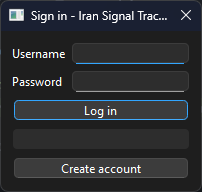
\includegraphics[width=0.5\linewidth]{fig_signin}
\caption{دروازه‌ی ورود برنامه‌ی نمونه}
\label{fig:signin}
\end{figure}

\section{داده‌های شبکه}
زبانه‌ی داده‌های شبکه (شکل
\autoref{fig:network})
هسته‌ی برنامه است: جدولی از نمونه‌های سیگنال با فیلترهای استان (با شهرهای آبشاری)، فناوری و اپراتور، جستجو، بازنشانی، خروجی
\lr{\gls{CSV}}
و نمودار ستونی میانگین کیفیت. برای مجموعه‌داده‌های بزرگ، جدول صفحه‌بندی می‌شود (اندازه‌های صفحه ۵۰ تا ۱۰۰۰) و نوار وضعیت همیشه اندازه‌ی کامل نتیجه را نشان می‌دهد.

\begin{figure}[H]
\centering
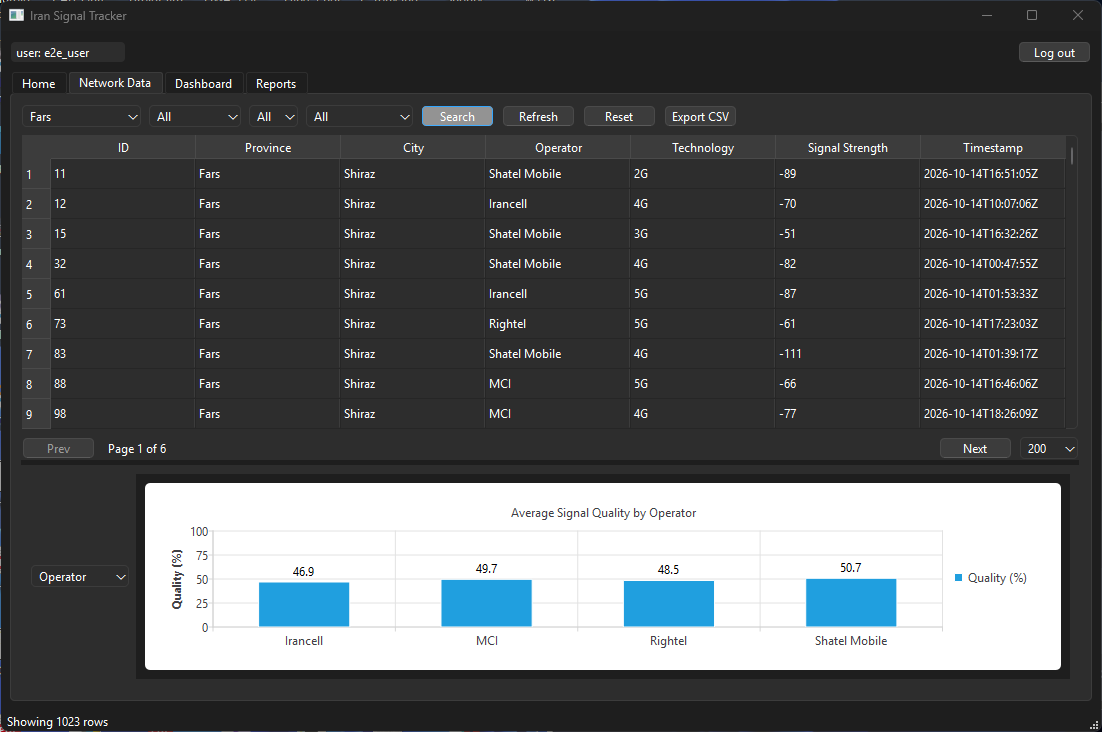
\includegraphics[width=\linewidth]{fig_network}
\caption{زبانه‌ی داده‌های شبکه؛ فیلتر استان فارس اعمال شده است}
\label{fig:network}
\end{figure}

\section{داشبورد و گزارش‌ها}
داشبورد (شکل
\autoref{fig:dashboard})
شاخص‌های کلیدی مانند میانگین کیفیت و تعداد نمونه‌ها، روند روزانه‌ی کیفیت، فهرست ضعیف‌ترین نمونه‌ها، نمودار دایره‌ای سهم اپراتورها و نمودار ستونی کیفیت بر حسب فناوری را نشان می‌دهد. هر دو نمودار جدید از فیلترهای همان زبانه تبعیت می‌کنند. زبانه‌ی گزارش‌ها (شکل
\autoref{fig:reports})
جدول خلاصه‌ی گروه‌بندی‌شده (بر اساس استان، اپراتور یا فناوری)، نمودار دایره‌ای سهم هر گروه، نمودار روند روزانه‌ی گروه انتخاب‌شده و خروجی
\lr{\gls{CSV}}
را ارائه می‌دهد.

\begin{figure}[H]
\centering
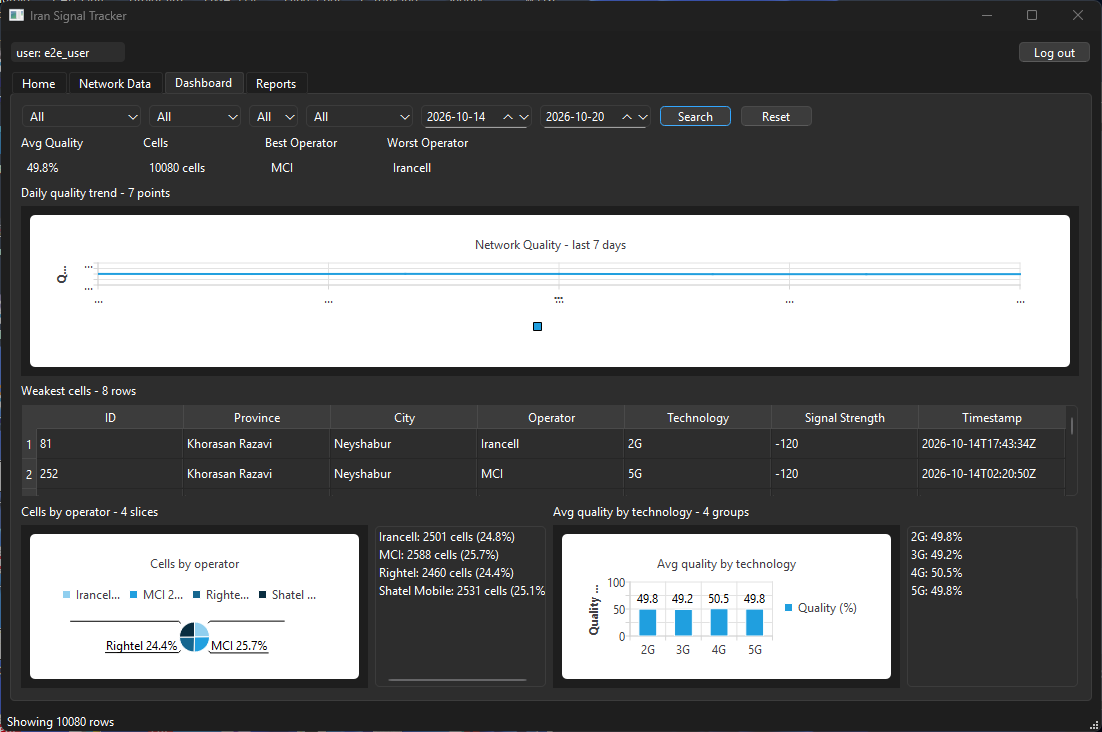
\includegraphics[width=\linewidth]{fig_dashboard}
\caption{داشبورد برنامه؛ نمودارهای دایره‌ای و ستونی سمت چپ و راست}
\label{fig:dashboard}
\end{figure}

\begin{figure}[H]
\centering
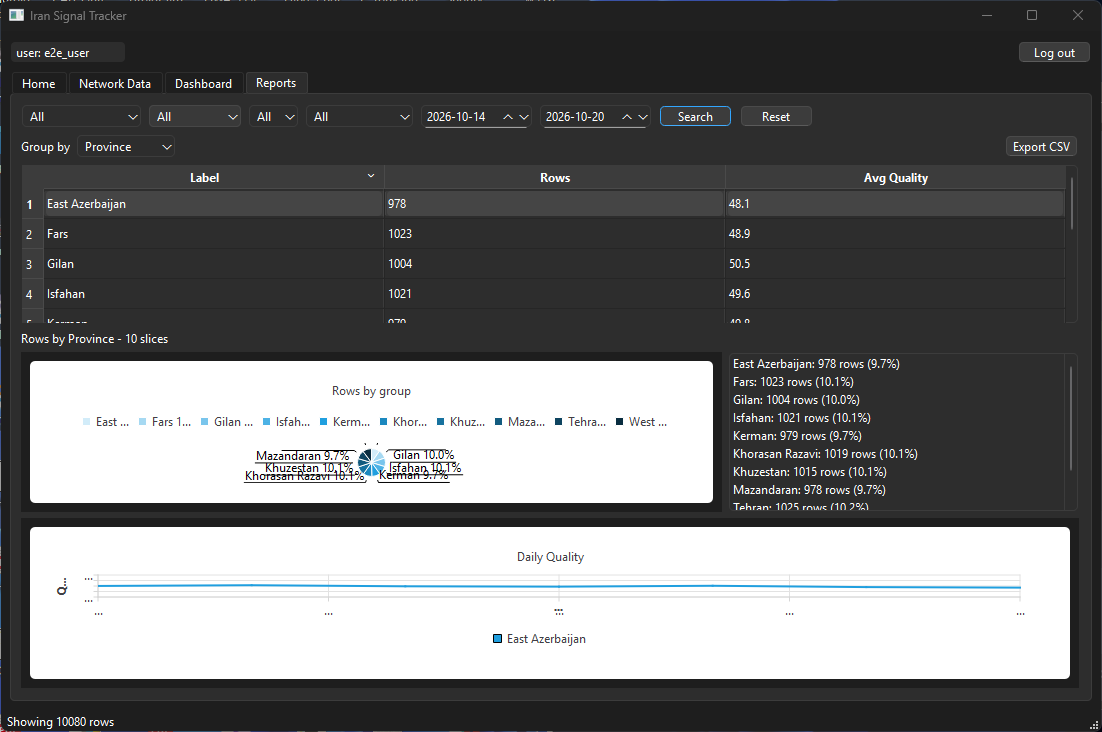
\includegraphics[width=\linewidth]{fig_reports}
\caption{زبانه‌ی گزارش‌ها؛ خلاصه‌ی گروه‌بندی‌شده، نمودار دایره‌ای و روند روزانه}
\label{fig:reports}
\end{figure}

\section{مجموعه‌داده}
داده‌ی برنامه یک مجموعه‌ی شبه‌واقعی از کیفیت سیگنال مخابراتی است: ۱۰٬۰۸۰ نمونه در بازه‌ی هفت روز (۱٬۴۴۰ نمونه در روز)، با تولید قطعی مبتنی بر بذر ثابت تا هر اجرا بازتولید‌پذیر باشد. داده‌ها شامل ده استان، شهرهای متناظر از نقشه‌ی دامنه‌ی برنامه، چهار اپراتور و چهار فناوری \lr{2G} تا \lr{5G} هستند. قدرت سیگنال هر نمونه به سنجه‌ی کیفیت ۰ تا ۱۰۰ درصد نگاشت می‌شود و همه‌ی نمودارها از این نگاشت مشترک تغذیه می‌کنند.

این برنامه آگاهانه ویژگی‌هایی را دارد که تست سرتاسری را دشوار می‌کند: جریان ورود با پنجره‌های متعدد، فیلترهای وابسته به هم، صفحه‌بندی، مجازی‌سازی جدول، نمودارهای گرافیکی که داده‌شان در درخت دسترس‌پذیری دیده نمی‌شود و دو نقش کاربری. همین دشواری‌ها معیار ارزیابی چارچوب در \autoref{chap:evaluation}
هستند.
\chapter{طراحی و پیاده‌سازی چارچوب}
\label{chap:framework}

این فصل هسته‌ی پایان‌نامه است: معماری لایه‌ای چارچوب، قراردادهای پایداری، لایه‌های مکان‌یابی، اشیای صفحه، زبان مخصوص دامنه، مدیریت درایور و پنجره‌ها، جداسازی داده و گزارش‌گیری. انگیزه‌ی هر تصمیم، یکی از دشواری‌های واقعی تست رابط کاربری است که در طول پیاده‌سازی مشاهده و مستند شد.

\section{نگاه کلی به معماری}
چارچوب از پنج لایه تشکیل شده که از بالا به پایین با هم صحبت می‌کنند و فقط لایه‌ی پایین‌تر با درایور سروکار دارد:
\begin{itemize}
	\item \textbf{تست‌ها:} سناریوهای رفتاری؛ تنها از لایه‌ی زبان دامنه استفاده می‌کنند و هیچ فراخوانی درایوری ندارند.
	\item \textbf{لایه‌ی زبان دامنه (\lr{\gls{DSL}}):} پوشش معنادار برنامه («واحد استان را فیلتر کن»، «مجموع برش‌های نمودار دایره‌ای را بخوان»).
	\item \textbf{لایه‌ی اشیای صفحه (\gls{PageObject}):} برای هر صفحه/زبانه یک کلاس؛ تنها نهاد همان صفحه را می‌شناسد.
	\item \textbf{لایه‌ی مکان‌یابی:} مکان‌یابی کنترل‌ها با استراتژی‌های چندگانه، نهان‌گاه دسته‌ها
	\gls{HandleCache}
	و جستجوی محدوده‌ای.
	\item \textbf{لایه‌ی درایور:} کارخانه‌ی درایور
	\gls{DriverFactory}،
	برپایی سرور، اجبار پیش‌زمینه و ورودی صفحه‌کلید سطح سیستم‌عامل.
\end{itemize}

این جداسازی مستقیماً از الگوی شیء صفحه می‌آید
\cite{fowler2002}
اما با یک قاعده‌ی سخت‌گیرانه‌تر تکمیل شده است: دایرکتوری تست‌ها در بازرسی خودکار به فراخوانی‌های درایور حساس است و وجود حتی یک فراخوانی خام، ساخت را می‌شکند. به این ترتیب مرز لایه‌ها قرارداد شفاهی نمی‌ماند.

\section{قراردادهای پایداری در برنامه}
شکننده‌ترین بخش تست‌های رابط کاربری، مکان‌یابی است. چارچوب دو قرارداد در سطح برنامه‌ی نمونه تعریف می‌کند که برنامه‌های هدف باید رعایت کنند:
\begin{enumerate}
	\item \textbf{شناسه پایدار
	\gls{StableIdentifier}:}
	هر کنترل تعاملی، نام دامنه‌ای ثابت خود را هم در
	\lr{objectName}
	(که در
	\lr{\gls{UIA}}
	\cite{uia}
	به
	\lr{AutomationId}
	می‌رسد) و هم در
	\lr{accessibleName}
	(که به
	\lr{Name}
	می‌رسد) قرار می‌دهد. مکان‌یابی ابتدا با نام و در صورت نیاز با شناسه انجام می‌شود.
	\item \textbf{قرارداد خوانش
	\gls{ReadoutContract}:}
	عناصر فقط‌خواندنی (نشانگرهای کلیدی، برچسب‌های شمارنده) شناسه‌ی پایدار خود را در
	\lr{objectName}
	نگه می‌دارند اما
	\lr{accessibleName}
	آن‌ها همیشه متن نمایش‌داده‌شده را منعکس می‌کند؛ زیرا هیچ کلید ویژگی‌ای در
	\lr{WinAppDriver}
	مقدار داخلی این کنترل‌ها را نمی‌خواند. نمودارهای گرافیکی نیز داده‌ی خود را در یک فهرست خوانا آینه می‌کنند تا تست‌ها به تصویر دسترسی نداشته باشند و به داده.
\end{enumerate}

با این دو قرارداد، تستِ نمودار و نشانگر \pdash{} که در درخت دسترس‌پذیری اصلاً دیده نمی‌شوند \pdash{} به تست داده‌ی خوانا تبدیل می‌شود و تست‌ها در برابر تغییرات ظاهری مقاوم می‌مانند.

\section{لایه‌ی مکان‌یابی و نهانگاه دسته‌ها}
هر جستجوی ریشه‌ای در
\lr{\gls{UIA}}
کل درخت را بازمی‌گردد؛ در برنامه‌ای با جدول ده‌هزار ردیفی، هر جستجو تا بیش از ده ثانیه طول می‌کشد. سه سازوکار پایداری و سرعت پیاده شد: نخست، برنامه‌ی هدف بخش‌های کوچک نام‌گذاری‌شده (نوار فیلتر، نوار صفحه‌بندی) را در درخت آشکار می‌کند و لایه‌ی مکان‌یابی جستجو را به همان محدوده‌ی کوچک محدود می‌کند (پردازش اندازه‌گیری‌شده: از ۱۱ ثانیه به ۰٫۰۲ ثانیه)؛ دوم، دسته‌ی \lr{(Handle)} هر کنترل پس از نخستین یافتن در نهانگاه
\gls{HandleCache}
با کلید (عنوان پنجره، شناسه کنترل) نگه داشته می‌شود و کار با دسته‌ی نهان‌شده در حد ۰٫۰۱ ثانیه است؛ سوم، نهانگاه در هر تغییر پنجره باطل می‌شود (بخش اتصال فازی).

\section{کارخانه‌ی درایور و اتصال فازی}
\lr{WinAppDriver}
جلسه را به یک پنجره‌ی سطح‌بالا گره می‌زند؛ برنامه‌ی نمونه در جریان ورود، پنجره‌ی ورود را می‌بندد و پنجره‌ی اصلی می‌سازد و همین تغییر، جلسه‌ی قدیم را بی‌اعتبار می‌کند. کارخانه‌ی درایور فرایند برنامه را مالکیت می‌کند (اجرای برنامه، پایان دادن به آن در پایان جلسه) و جلسه را به عنوان پنجره‌ی سطح‌بالای برنامه می‌سازد؛ لایه‌ی زبان دامنه در هر فاز (ورود، پنجره اصلی) دوباره به پنجره‌ی جاری متصل می‌شود؛ به این سازوکار «اتصال فازی»
\gls{PhaseAttach}
گفته می‌شود. علاوه بر این، دو رفتار خطرناک ویندوز مهار شده است: اول اینکه ورودی صفحه‌کلید به پنجره‌ی پیش‌زمینه می‌رسد و اگر برنامه در پیش‌زمینه نباشد، متن تست در پنجره‌ی دیگری (مثلاً یک پنجره گفتگو) تایپ می‌شود؛ کارخانه پیش از هر تعامل، پیش‌زمینه را به‌صورت قطعی به برنامه منتقل می‌کند. دوم اینکه
\lr{send\_keys}
درایور به متن اضافه می‌کند نه جایگزین؛ اشیای صفحه ورودی‌های متنی را پیش از تایپ خالی می‌کنند.

\section{ورودی صفحه‌کلید و اجرای قطعی}
تعامل با چرخاننده‌ها (کمبوها) از مسیر صفحه‌کلید انجام می‌شود: باز کردن پنجره‌ی بازشو با کلیک، تایپ سطح سیستم‌عامل متن گزینه (به‌کارافتادن جستجوی نوع‌نویسی
\lr{Qt})
و تأیید با
\lr{Enter}.
این مسیر نه به مکان‌یابی عناصر پنجره‌ی بازشو نیاز دارد و نه در برابر هم‌نامی گزینه‌ها با سلول‌های جدول می‌شکند. همین الگو برای فیلترهای تاریخ تعمیم داده شد: تاریخ با ارسال هشت رقم از طریق خود درایور روی عنصر تاریخ تنظیم می‌شود و بخش‌های سال، ماه و روز به‌ترتیب پر می‌شوند. هر یک از این روش‌ها با یک تست کاوشی
\lr{(probe)}
به صورت مستقل کشف و در توضیحات کد مستند شده است.

\section{تست با زبان دامنه در برابر کد خام درایور}
برای نشان‌دادن ارزش لایه‌ی زبان دامنه، همان سناریو را در دو سطح می‌بینیم. کد زیر همان تعامل با فراخوانی‌های خام درایور است؛ یعنی آنچه نویسنده‌ی تست بدون چارچوب می‌نویسد:

\begin{latin}
\begin{lstlisting}[language=Python]
# raw driver access - what a tester writes WITHOUT the framework
driver = attach("Iran Signal Tracker")
section = driver.find_element(
    "xpath", "//*[@AutomationId='dashboardFilterSection']")
combo = section.find_element(
    "xpath", ".//*[@AutomationId='dashboardProvinceCombo']")
combo.click(); sleep(0.5)      # popup takes keyboard focus
keyboard.type_text("Tehran"); keyboard.press_enter()
sleep(0.6)                     # cascade settle
driver.find_element(
    "xpath", "//*[@Name='dashboardSearchButton']").click()
kpi = driver.find_element(
    "xpath", "//Edit[contains(@AutomationId,'kpiCells')]")
assert kpi.get_attribute("Name") == "1023 cells"
\end{lstlisting}
\end{latin}

و این همان تست با زبان دامنه‌ی چارچوب:

\begin{latin}
\begin{lstlisting}[language=Python]
dash = signed.dashboard()
dash.province("Tehran").search()
assert dash.kpi("cells") == "1023 cells"
\end{lstlisting}
\end{latin}

تفاوت فقط کوتاه‌تر شدن کد نیست. در نسخه‌ی خام، نویسنده‌ی تست باید بداند مکان‌یابی با کدام استراتژی کار می‌کند، چرا بین کلیک و تایپ مکث لازم است، چرا ورودی باید از مسیر صفحه‌کلید سیستم‌عامل برود، و ده‌ها رفتار ریز زیرساخت که در جدول
\autoref{tab:quirks}
فهرست شده‌اند؛ هر خطای ریز در این جزئیات، شکست نمایشیِ تست است نه شکست برنامه. در نسخه‌ی زبان دامنه، همه‌ی آن دانش یک بار در لایه‌ی اشیای صفحه زیست می‌کند و نویسنده‌ی تست با واژگان دامنه («استان»، «جستجو»، «خواندن نشانگر») کار می‌کند؛ اگر فردا جستجو از مسیر دیگری انجام شود، فقط یک کلاس تغییر می‌کند و هیچ تستی بازنویسی نمی‌شود. به بیان دیگر، نسخه‌ی خام دانش فنی را در همه‌جا پخش می‌کند و نسخه‌ی زبان دامنه آن را یک‌جا متمرکز می‌کند؛ همین تمرکز است که نگهداشت مجموعه‌ی ۲۵ سناریویی را برای یک نفر ممکن می‌کند.

\section{جداسازی پایگاه‌داده در سطح تست}
تست‌ها باید مستقل و بازتولیدپذیر باشند
\cite{meszaros2007}.
هر تست پیش از اجرا، فایل پایگاه‌داده‌ی خود را از یک «فیکسچر ثابت»
\gls{Fixture}
از پیش متعهدشده بازمی‌گرداند و سپس مهاجرت‌های طرح را روی آن اعمال می‌کند. نگاشت تست به فیکسچر در یک فایل پیکربندی است و بازگردانی بی‌قیدوشرط است (نه «فقط اگر تغییر کرده») تا هیچ تستی به حالت جلسه‌ی قبلی وابسته نماند. خروجی‌های
\lr{\gls{CSV}}
نیز در هر تست پاک می‌شوند تا تست‌های گزارش‌گیری به فایل‌های باقی‌مانده از اجرای دیگر تکیه نکنند.

طراحی فیکسچرها عمداً چندپایگاه‌داده‌ای است: هر فیکسچر یک فایل
\lr{SQLite}
متعهدشده با محتوای قطعی است و فایل پیکربندی
\lr{JSON}
تعیین می‌کند هر تست کدام فیکسچر را دریافت کند؛ در حالت پیش‌فرض همه‌ی تست‌ها فیکسچر کامل با ۱۰٬۰۸۰ نمونه می‌گیرند و هر تست می‌تواند با یک نگاشت صریح فیکسچر خود را بازنویسی کند. چارچوب هم‌اکنون دو فیکسچر دارد: کامل و خالی (برای رفتار برنامه با داده‌ی صفر)، و افزودن فیکسچر تازه — مثلاً داده‌ی یک استان خاص برای تست‌های آینده — تنها یک فایل
\lr{.db}
و یک خط در فایل پیکربندی است؛ هیچ تغییری در کد چارچوب لازم نیست. فایل نگاشت چنین است:

\begin{latin}
\begin{lstlisting}[numbers=none]
{
  "default": "seed_full",
  "tests/test_tc018_empty_fixture.py::test_tc018_empty_fixture":
    "empty"
}
\end{lstlisting}
\end{latin}

کلید نخست، فیکسچر پیش‌فرض همه‌ی تست‌ها را تعیین می‌کند و هر کلید دیگر یک پوشش سرتاسری است: شناسه‌ی کامل تست (مسیر فایل + نام تابع) به فیکسچر موردنظر نگاشت می‌شود. این شکست «پیکربندی به جای کد» باعث می‌شود انتخاب داده‌ی هر تست در یک نگاه دیده و تغییرش بدون دست زدن به آزمون انجام شود. فیکسچرها هرگز در محل اجرا باز نمی‌شوند (فقط بازنویسی بایت‌به‌بایت) تا بایت‌های فایل متعهدشده سالم بمانند و نتیجه‌ی هر اجرا دقیقاً بازتولید شود.

\section{گزارش‌گیری و سوییت‌ها}
تست‌ها در فایل‌های مستقل به نام سناریو (از
\lr{TC001}
تا
\lr{TC025})
نوشته شده‌اند و فایل پیکربندی سوییت‌ها، نام هر سوییت (\lr{smoke}، \lr{auth}، \lr{filters}، \lr{reporting}، \lr{dashboard}، \lr{data}، \lr{unit}) را به فهرست فایل‌های تست آن نگاشت می‌کند. اسکریپت اجرا، پیش از اجرا از سلامت ساختمان برنامه و سرور درایور پیش‌پرواز می‌گیرد، مجموعه را اجرا می‌کند و در پایان گزارش
\lr{Allure}
\cite{allure}
را بسازد و روی یک سرور محلی باز کند؛ زیرا باز کردن گزارش از مسیر فایل، نسخه‌های جدید گزارش را می‌شکند. تصویر لحظه‌ی خطا نیز به صورت خودکار به گزارش هر تست شکست‌خورده پیوست می‌شود. فایل نگاشت سوییت‌ها نمونه‌ای واقعی از همین پیکربندی است:

\begin{latin}
\begin{lstlisting}[numbers=none]
{
  "smoke":  ["test_tc001_launch", "test_tc012_login",
             "test_tc002_province_filter", "test_tc009_export_csv"],
  "auth":   ["test_tc011_register", "test_tc012_login",
             "test_tc013_logout", "test_tc015_users_admin"],
  "filters": ["test_tc002_province_filter",
              "test_tc003_city_filter", "..."],
  "reporting": ["test_tc009_export_csv",
                "test_tc010_chart_visibility", "..."],
  "dashboard": ["test_tc020_dashboard_filters",
                "test_tc021_dashboard_pie_vs_csv",
                "test_tc022_dashboard_tech_bar"],
  "data":  ["test_tc008_refresh", "test_tc016_pagination",
            "test_tc019_demo_failure", "..."],
  "unit":  ["test_fixtures_unit"]
}
\end{lstlisting}
\end{latin}

هر نام سوییت به فهرست فایل‌های تست خود نگاشت می‌شود (پسوند
\lr{.py}
اختیاری است) و اسکریپت اجرا با یک نام، آن سوییت را اجرا می‌کند؛ انتخاب سوییت در هنگام اجرا (مثلاً فقط
\lr{auth}
در هر تغییر پوشش احراز هویت) بدون هیچ تغییری در کد ممکن است. این فایل در عمل نقش فهرست وام‌های کیفیت را دارد: هر سناریو دقیقاً در یک سوییت ثبت است و جابه‌جایی آن بین سوییت‌ها یک خط تغییر است.

\section{سوت‌های مستندشدهی زیرساخت}
در طول پیاده‌سازی، رفتارهای غیرمنتظره‌ای از زیرساخت مشاهده و هر یک با تست کاوشی مستند شد. جدول
\autoref{tab:quirks}
خلاصه‌ی آن‌هاست؛ ارزش این جدول در این است که هر یک به یک سازوکار دائمی در چارچوب تبدیل شده است.

\begin{table}[H]
\centering
\caption{سوت‌های مشاهده‌شدهی زیرساخت و پاسخ چارچوب}
\label{tab:quirks}
\begin{tabularx}{\textwidth}{@{}XX@{}}
\hline
رفتار مشاهده‌شده & پاسخ چارچوب \\
\hline
\lr{send\_keys}
به متن اضافه می‌کند & پاک‌سازی پیش از تایپ در اشیای صفحه \\
جلسه به یک پنجره گره می‌خورد & اتصال فازی + باطل‌سازی نهانگاه \\
کلیک به پنجره‌ی غیرپیش‌زمینه می‌رسد & اجبار قطعی پیش‌زمینه \\
جستجوی ریشه‌ای بسیار کند & بخش‌های نام‌گذاری‌شده + نهانگاه دسته‌ها \\
عناصر جدول مجازی می‌شوند & شمارش از برچسب‌ها نه از ردیف‌ها \\
داده‌ی نمودار در درخت دیده نمی‌شود & قرارداد خوانش و فهرست آینه \\
\hline
\end{tabularx}
\end{table}

نمونه‌ی زیر تستی است که تنها با زبان دامنه نوشته شده؛ خوانایی و نبودِ هر فراخوانی درایوری معیار طراحی این لایه است:

\begin{latin}
\begin{lstlisting}[language=Python]
def test_tc021_dashboard_pie_vs_csv(signed):
    net = signed.network()
    net.province("Tehran")
    result = net.export().should_create_file()
    per_operator = count_operators(result.newest_file())

    dash = signed.dashboard()
    dash.province("Tehran").search()
    slices = dash.pie_slices()
    assert {label: count for label, count, _ in slices} \
        == dict(per_operator)
\end{lstlisting}
\end{latin}
\chapter{ارزیابی و نتایج}
\label{chap:evaluation}

در این فصل چارچوب بر معیارهای عملی ارزیابی می‌شود: پوشش سناریوها، نتیجه‌ی اجرای کامل، گزارش‌گیری و مسیر انتقال به پایپلاین‌ی
\lr{\gls{CI}}/\lr{\gls{CD}}.

\section{محیط آزمایش}
همه‌ی ارزیابی روی یک سامانه‌ی ویندوزی واقعی انجام شده است؛ مشخصات محیط به پیروی از رویه‌ی گزارش‌های مهندسی، فهرست‌وار آورده می‌شود:
\begin{itemize}
	\item سیستم‌عامل: ویندوز ۱۱ (میزکار) با فعال‌بودن حالت توسعه‌دهنده
	\item زبان و کیت برنامه‌ی نمونه:
	\lr{Qt 6.8.3 (MinGW 13.1), CMake, Ninja}
	\item زبان چارچوب:
	\lr{Python 3.12}
	با
	\lr{pytest}
	و
	\lr{Appium Python Client}
	\item سرور درایور:
	\lr{Appium 3}
	روی درگاه ۴۷۲۳ و
	\lr{WinAppDriver}
	برای مسیر اجرای بی‌سر
	\gls{HeadlessRun}
	\item گزارش‌ساز:
	\lr{Allure 3}
	\item سخت‌افزار: رایانه‌ی شخصی با پردازنده‌ی
	\lr{x86\_64}
	و ۱۶ گیگابایت حافظه
\end{itemize}

\section{سوییت سناریوها}
۲۵ سناریوی سرتاسری نوشته شده که به شش خانواده تقسیم می‌شوند: جریان ورود و ثبت‌نام (۵ سناریو)، فیلترهای جدول شبکه (۶ سناریو)، صفحه‌بندی و شناسه‌ی ردیف‌ها (۳ سناریو)، داشبورد (۴ سناریو شامل سنجش نمودار دایره‌ای و ستونی در برابر داده‌ی مستخرج از خروجی
\lr{\gls{CSV}})،
گزارش‌ها (۴ سناریو شامل انتقال فیلتر و گروه‌بندی) و تست‌های زیرساخت (۲ سناریو). در کنار این‌ها، دو تست داخلی برنامه (تست دود رابط کاربری و تست لایه‌ی داده) و یک سناریوی نمایشی عمداً شکست‌خورده وجود دارد که نقش آن، نشان‌دادن رفتار گزارش‌گیری در هنگام خطا در جلسه‌ی نمایش است.

نکته‌ی مهم در سناریوهای نمودار این است که تست، خروجی
\lr{\gls{CSV}}
همان فیلتر را از زبانه‌ی شبکه استخراج و توزیع داده را مستقل از برنامه محاسبه می‌کند؛ سپس برش‌های خوانده‌شده از فهرست آینه‌ی نمودار را با آن مقایسه می‌کند. به این ترتیب درستیِ نمودار با «منبع حقیقت دیگری» سنجیده می‌شود نه با خود برنامه.

\section{اجرای کامل و گزارش}
اجرای کامل مجموعه در حدود شش دقیقه انجام می‌شود؛ خروجی پایدار آن ۲۴ سناریوی موفق و یک شکست عمدی است. گزارش
\lr{Allure}
این اجرا در شکل
\autoref{fig:allure}
نمایش داده شده است: شمار کل، موفق و شکست به تفکیک فایل سناریو، با زمان‌بندی هر تست. در صورت شکست هر تست، تصویر لحظه‌ی خطا به گزارش پیوست می‌شود.

\begin{figure}[H]
\centering
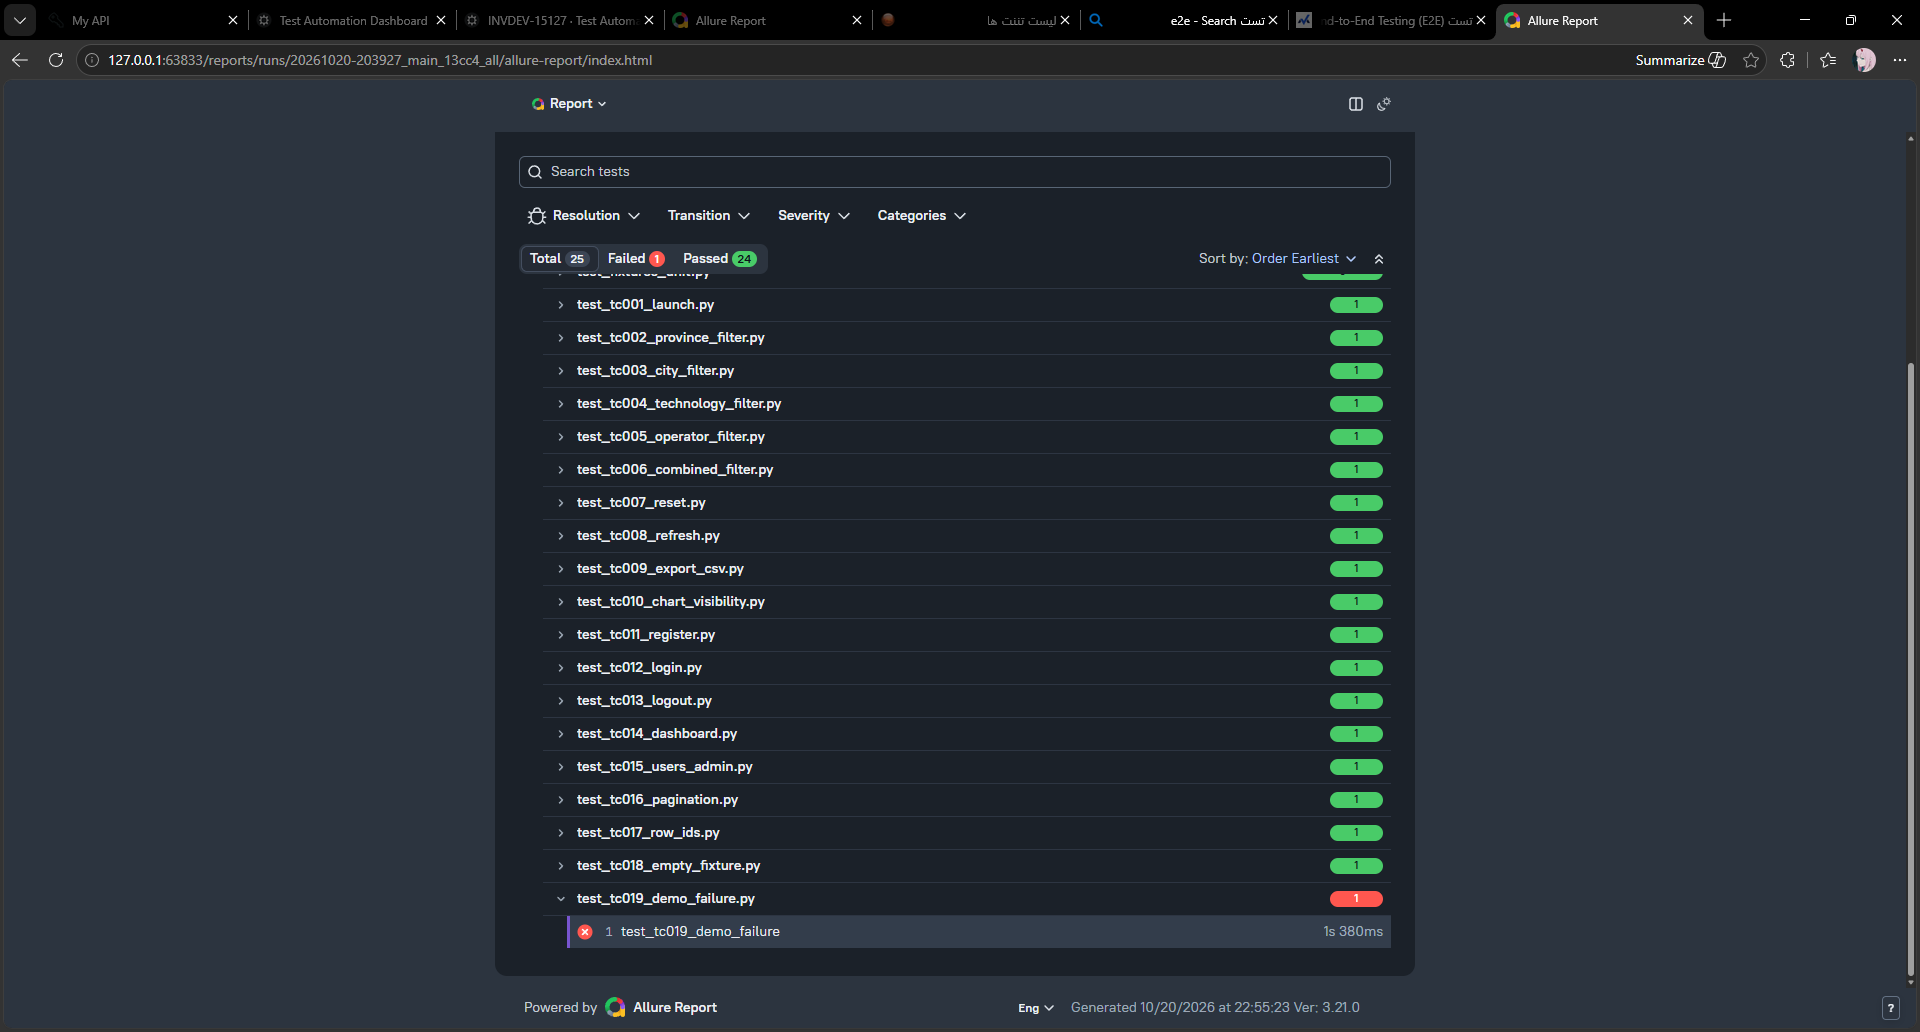
\includegraphics[width=\linewidth]{fig_allure}
\caption{گزارش \lr{Allure} پس از اجرای کامل مجموعه؛ شکست عمدی سناریوی نمایشی آشکار است}
\label{fig:allure}
\end{figure}

برای نشان‌دادن جریان کامل اجرا، یک فیلم کوتاه از اجرای کل مجموعه ضبط شده است. در نسخه‌ی الکترونیکی این پایان‌نامه، ویدیوی زیر با کلیک فعال می‌شود:

\begin{figure}[H]
\centering
\includemedia[
	width=0.9\linewidth,
	height=0.51\linewidth,
	activate=pagevisible,
	addresource=fig_suite_run.mp4,
	flashvars={source=fig_suite_run.mp4&autoPlay=false&loop=true}
]{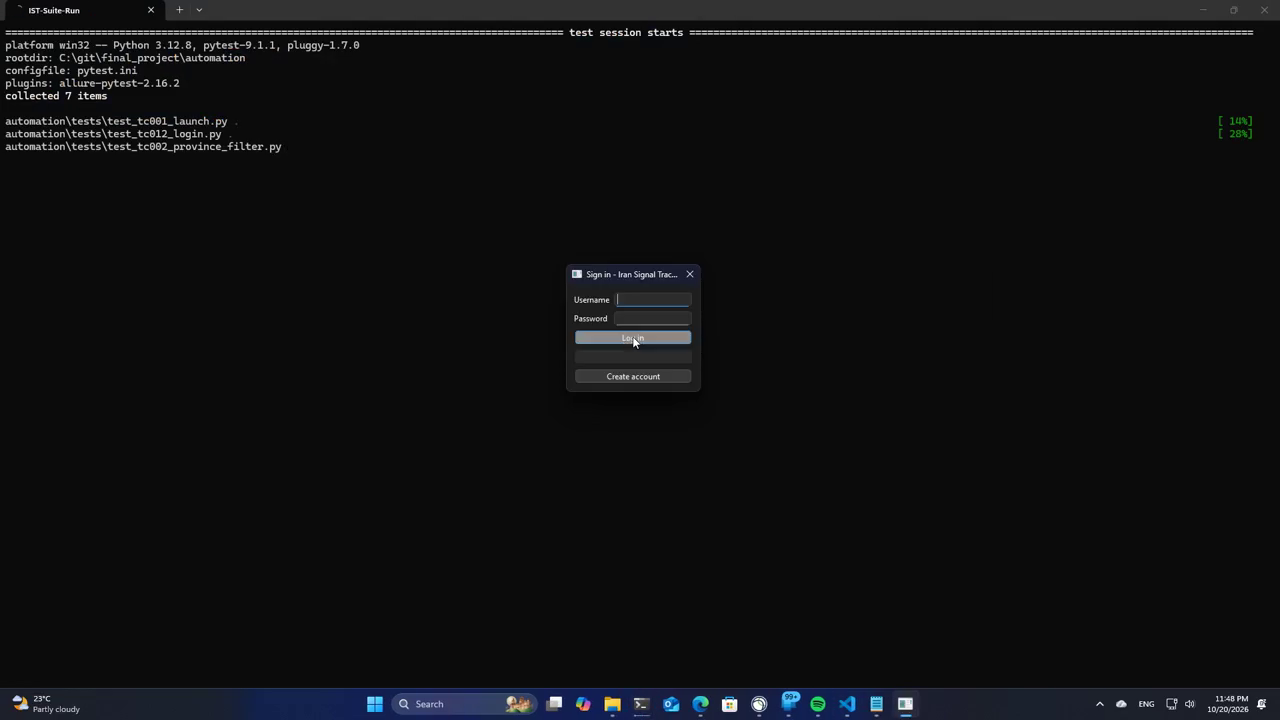
\includegraphics[width=0.9\linewidth]{fig_suite_poster}}{VPlayer.swf}
\caption{فیلم اجرای کامل سوییت سرتاسری (نیازمند نمایشگر \lr{PDF} تعاملی)}
\label{fig:video}
\end{figure}

در نسخه‌ی چاپی، شکل‌های
\autoref{fig:signin}
تا
\autoref{fig:allure}
در فصل‌های قبلی جریان را بازگو می‌کنند.

\section{انتقال به پایپلاین \lr{CI/CD}}
چارچوب از ابتدا برای سوار‌شدن بر پایپلاین طراحی شده است. شکل هدف پایپلاین چنین است:
\begin{latin}
\begin{lstlisting}[language=bash, numbers=none]
Commit
  -> Build App        (cmake configure + build; ctest smoke + db_test gate)
  -> Launch Appium    (appium server on :4723)
  -> Launch Application (driver factory starts the exe via caps)
  -> Execute Tests    (python -m pytest automation/tests)
  -> Generate Allure  (allure generate ... -o reports/allure-report)
  -> Publish Report   (host allure-report artefact, if: always())
\end{lstlisting}
\end{latin}

نکات طراحی‌شده برای نویسنده‌ی پایپلاین: نهان‌گاه کردن مسیرهای
\lr{Qt}
،
\lr{MinGW}
و
\lr{Python}
بر اساس پین‌های نسخه در مستندات محیط؛ نیاز رانر به ویندوز، حالت توسعه‌دهنده و نصب
\lr{WinAppDriver}؛
شکست هر تست به معنی شکست کار بدون حذف انتشار گزارش (با شرط
\lr{always()})
؛ و مسیر اجرای بی‌سر با
\lr{DRIVER\_MODE=direct}
که سرور
\lr{Appium}
را از معادله حذف می‌کند و مستقیماً به
\lr{WinAppDriver}
وصل می‌شود. جداسازی پایگاه‌داده در سطح تست (فصل
\autoref{chap:framework})
ضمانت می‌کند که اجراهای موازی‌نما و متوالی روی یک رانر، به هم آلودگی ایجاد نکنند.

\section{تحلیل نتایج}
سه شاهد کیفی از ارزیابی قابل استناد است. نخست، پایداری: کل مجموعه در چندین اجرای پیاپی با همان نتیجه اجرا شده و تنها شکست‌ها، شکست عمدی سناریوی نمایشی بوده است. دوم، سرعت: با بخش‌بندی درخت مکان‌یابی و نهانگاه دسته‌ها، زمان اجرای کامل از حدی که عملاً غیرقابل‌استفاده بود (جستجوهای تک‌ثانیه‌ای تا ۱۱ ثانیه) به حدود شش دقیقه برای ۲۵ سناریو رسید. سوم، نگهداشت‌پذیری: در طول توسعه، تغییرات متعددی در چیدمان رابط کاربری برنامه (جابه‌جایی پنل‌ها، افزودن نمودار) رخ داد که هیچ‌یک تستی را نشکست؛ تنها لایه‌ی اشیای صفحه تغییر کرد — همان چیزی که جداسازی لایه‌ها وعده می‌داد. محدودیت‌های چارچوب نیز روشن است: وابستگی به ویندوز و
\lr{WinAppDriver}،
نیاز برنامه‌های هدف به رعایت قراردادهای پایداری، و اجرای تعاملی (نه هم‌زمان) برای درایورهای پنجره‌ای.
\chapter{نتیجه‌گیری و کارهای آینده}
\label{chap:conclusion}

\section{نتیجه‌گیری}
در این پایان‌نامه یک چارچوب تست سرتاسری متن‌باز برای نرم‌افزارهای مبتنی بر
\lr{Qt C++}
در بستر ویندوز طراحی و پیاده‌سازی شد. چارچوب روی زیرساخت استاندارد
\lr{WinAppDriver}/\lr{Appium}
سوار است و آنچه این زیرساخت نمی‌دهد — پایداری، خوانایی و نگهداشت‌پذیری تست‌ها — را با پنج لایه‌ی معماری می‌سازد: لایه‌ی مکان‌یابی با نهانگاه دسته‌ها و جستجوی محدوده‌ای، لایه‌ی اشیای صفحه، لایه‌ی زبان مخصوص دامنه، کارخانه‌ی درایور با اتصال فازی، و لایه‌ی جداسازی داده و گزارش‌گیری. دو قرارداد پایداری (شناسه پایدار و قرارداد خوانش) رابطه‌ی برنامه‌ی هدف و چارچوب را قواعد‌مند می‌کند و تستِ نمودارهای گرافیکی را — که در درخت دسترس‌پذیری دیده نمی‌شوند — به تست داده‌ی خوانا تبدیل می‌کند.

ارزیابی روی برنامه‌ی نمونه‌ای پیچیده (جریان ورود چندپنجره‌ای، فیلترهای آبشاری، صفحه‌بندی، مجازی‌سازی جدول، نمودار و گزارش‌گیری) با ۲۵ سناریوی سرتاسری انجام شد؛ اجرای کامل پایدار، بازتولیدپذیر و در حدود شش دقیقه است و گزارش تعاملی
\lr{Allure}
با پیوست تصویر خطا تولید می‌شود. جداسازی پایگاه‌داده در سطح تست، استقلال و بازتولیدپذیری سناریوها را تضمین می‌کند و مسیر انتقال به
\lr{\gls{CI}}/\lr{\gls{CD}}
به‌صورت طراحی‌شده آماده است. همه‌ی اجزا متن‌باز و بدون هزینه‌ی مجوز هستند.

\section{کارهای آینده}
مسیر پیش‌روی چارچوب در چهار جهت است:
\begin{itemize}
	\item \textbf{اجرا در پایپلاین:} برپایی رانر ویندوزی، نهان‌گاه وابستگی‌ها و انتشار خودکار گزارش پس از هر تغییر؛ مسیر اجرای بی‌سر با
	\lr{DRIVER\_MODE=direct}
	آماده است.
	\item \textbf{گسترش پلتفرم:} افزودن درایورهای دیگر از الگوی کارخانه (
	\lr{Linux}
	با
	\lr{AT-SPI}،
	مک با
	\lr{Accessibility API})
	بدون تغییر لایه‌های بالا؛ قراردادهای پایداری مستقل از پلتفرم‌اند.
	\item \textbf{تولید خودکار تست:} استفاده از بازشماری کنترل‌های برنامه (ابزار بازرسی موجود در چارچوب) برای پیشنهاد اسکلت سناریوها و کشف انحراف شناسه‌ها در زمان ساخت برنامه.
	\item \textbf{تحلیل نتایج در گذر زمان:} نگهداری روند زمان اجرا و نرخ شکست اجراها برای آشکارسازی تست‌های شکننده پیش از آنکه تبدیل به مزاحم شوند.
\end{itemize}

\bibliography{./ETC/myref}
\printglossary

\clearpage
\begin{latin}
\section*{Abstract}

Automated UI testing for Qt C++ desktop applications has largely been limited to commercial tools; existing open-source options provide only raw infrastructure (a driver and a protocol) without architectural layers. This thesis presents the design and implementation of an open-source End-to-End (E2E) testing framework for Qt-based Windows desktop applications. The framework builds on WinAppDriver/Appium and adds five architectural layers: element location with a handle cache and scoped finds, page objects, a domain-specific language, a driver factory with phase attachment, and database isolation with reporting. Two stability contracts (stable identifiers and the readout contract) formalize the relationship between the target application and the framework, turning the testing of graphical charts into testing readable data.

For evaluation, a demo application, the Iran Signal Tracker (Qt and SQLite based), was built with deliberately hard-to-test flows: multi-window authentication, cascading filters, pagination, table virtualization, charts, and reporting. Twenty-five E2E scenarios were implemented; the full run is stable, reproducible, and completes in about six minutes, producing an interactive Allure report with failure screenshots. A CI/CD migration path is also designed.

\vskip 5mm
\textbf{Key Words}: End-to-End Testing, UI Automation, Qt, WinAppDriver, Appium, Domain-Specific Language, Page Object

\end{latin}
\newpage
\pagestyle{empty}
\begin{latin}
	\ignorespaces
	\begin{center}
		\begin{table}
			\begin{tabular}{ccc}
				& 
\includegraphics[trim={4cm 3cm 4cm 0.3cm},clip,width=0.24\linewidth]{Logo/En} & \\
				&
				\begin{minipage}{0.55\linewidth}
					\vskip 0.6cm
					\begin{center}
						School of Computer Engineering\\ [0.4cm]
					\end{center}
				\end{minipage}
				&
			\end{tabular}
		\end{table}
		\vspace*{\stretch{1}}
		\textbf{{\fontsize{15pt}{50pt}\selectfont Design and Implementation of an End-to-End Testing Framework for Qt C++ Applications}}
		\vspace*{\stretch{1}}
		\vskip 1cm
		\large{Bachelor's Thesis}\\[.4cm]
		\large{In the field of Computer Engineering}
		\vspace*{\stretch{1}}
		\vskip 1cm
		\Large{\textbf{Alireza BayatKhani}}
		\vskip 1.5cm
		\Large{Advisor}
		\\ [0.1cm] \Large{Dr. Abolfazl Dianat}\\
		\vskip 2cm
		\large{Autumn 2026}
	\end{center}
	\clearpage
\end{latin}
\end{document}